\documentclass[a4paper,oneside,12pt]{report}

\usepackage{custom}
\newcommand{\barg}{\si{\bar}\text{g}} 

\usepackage{fancyhdr} 
\fancyhf{}   
\fancyfoot[C]{\thepage}                     
\renewcommand\headrulewidth{0pt}
\pagestyle{fancy}

\begin{document}

\begin{titlepage}
\hfill

\begin{center}
\Huge
\textbf{LMECA1210 - Projet en construction mécanique 1\\}
\vspace{0.5cm}
\huge
\textbf{Dimensionnement d'une bielle\\}
\Large
\vspace{0.5cm}
\textbf{année académique 2014-2015\\}
\vspace{0.5cm}
\begin{figure}[b!]
	\center
	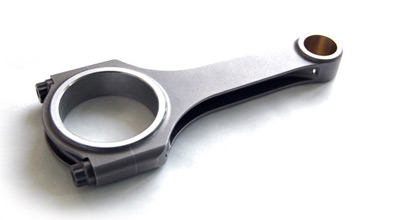
\includegraphics[width=12cm]{bielle.jpg}
\end{figure}

\end{center}
\begin{figure}[b!]
\begin{Large}
	Groupe 1\\
\end{Large}
	CHANDELLE François, 3673-13-00\\
	DISPAS David, 7189-12-00\\
	PAQUET Arnaud, 3668-13-00\\
	\\
	\newline
	\center
	
\includegraphics[width=7cm]{epl-logo.jpg}
\end{figure}
\end{titlepage}


\chapter{Réponse aux questions}

%Le fonctionnement d'un moteur à explosion repose sur la conversion du mouvement alternatif du piston en %rotation du vilebrequin. Cela se fait par l'intermédiaire d'une bielle. Cette pièce, répétant un cycle à %raison de plusieurs milliers de fois par minute, subit des forces conséquentes. Il est donc primordial %d'en faire l'analyse afin de prévoir sa forme optimale et les efforts maximaux à devoir supporter. 

\section{Mesures}

Le mécanisme qui nous intéresse est un système regroupant piston, bielle et manivelle. Notre groupe ayant reçu le vilebrequin d'une Audi A4 lors des séances de mesures, nous traiterons ici en particulier du moteur de cette voiture. De nos mesures, nous avons pu déduire la longueur R de la manivelle. Les groupes 12 et 16 nous ont donné respectivement la longueur de la bielle, L, et les longueurs des axes du piston (celui ci a en effet ici une forme elliptique). Le grand axe du piston est égal à l'alésage D des cylindres. Il est possible de trouver la cylindrée unitaire $V_c$ grâce à la formule suivante: 
$V_c =\frac{\pi D^2 R}{2}$

En multipliant ce volume par quatre, le nombre de cylindres, nous obtenons la cylindrée du moteur. Les valeurs réelles de R, D et $V_c$ nous ont été fournies dans un document annexe. Nous utiliserons ces données pour bénéficier d'une plus grande précision.\\

Pour finir, ne connaissant pas précisément le modèle de la voiture, nous ne pouvons qu'estimer le taux de compression, qui désigne le rapport du volume de la chambre de combustion lorsque le piston est au point minimum (en bas) sur le volume au point maximum (en haut). Une voiture dont le moteur fonctionne au diesel, a un taux de compression assez haut. Pour une audi A4, il avoisine 19.5 dans le cas d'une cylindrée égale à 1896 (comme pour la série
B5\footnote{\url{http://www.auto-data.net/en/?f=showCar&car_id=4416}}). Le résumé des mesures se trouve dans le tableau ci-dessous (voir figure 1.2).

\begin{figure}[h]
\centering
\begin{tabular}{|l|c|c|c|}
  \hline
  Longueur mesurée & Abréviation & Mesure & Distance réelle\\
  \hline
  Grand axe du piston & D & $79.4mm$ & $79.5mm$ \\
  Rayon de manivelle & R & $47mm$ & $47.75mm$\\
  Longueur de la bielle & L & $199.5mm$ & (non donné)\\
  Cylindrée unitaire & $V_c$  & $465cc$ & $474cc$\\
  Taux de compression & $\tau$ & / & $19.5$\\
  \hline
\end{tabular}
\caption{Les différentes mesures}
\end{figure}

\section{Evolution de la pression dans le cylindre}

L'analyse de l'évolution de la pression dans le cylindre se fait grâce à l'équation bien connue du premier principe de la thermodynamique. Divisée par la différentielle de l'angle du vilebrequin, d$\theta$, et simplifiée, nous obtenons:
$$\frac{dp}{d\theta}=-\gamma\frac{p}{V}\frac{dV}{d\theta}+(\gamma - 1) \frac{1}{V}\frac{dQ}{d\theta}$$
Nous avons choisi d'utiliser une méthode de Runge-Kutta d'ordre 2 pour intégrer numériquement cette équation. Cela ne se révèle utile que pour la phase de combustion, la seule où il y a un apport de chaleur non négligeable. Celui-ci est égal à $Q_{tot}=1650[kJ/kg] * V_{max} * \rho_{air}$. Les autres transformations sont considérées adiabatiques et la pression est trouvée simplement en considérant $PV^{\gamma}$ constant. L'échappement se fait avec un terme de relaxation $\frac{dp}{d\theta}=-k(p-p_atm)$ où $k=2,5$ pour que la pression retombe à 1 bar après une rotation du vilebrequin d'environ 30\degre.

\begin{figure}[H]
	\center
	\includegraphics[scale=0.6]{pression.jpg}
	\caption{Pression lors d'un cycle}
\end{figure}

\section{Efforts sur la bielle}

Le bilan des efforts sur la tête et le pied de bielle se mesure avec les deux formules ci-dessous. 

$$F_{pied} = \frac{\pi D^2}{4}p(\theta) -  m_{piston}R\omega^2 \cos(\theta) \qquad
F_{tete} = -\frac{\pi D^2}{4}p(\theta) +  (m_{piston}+m_{bielle})R\omega^2 \cos(\theta)$$

Voici les graphes représentant les efforts sur la bielle en fonction de l'angle du vilebrequin, à deux vitesses angulaires précises ($2500rpm$ et $4000rpm$):


\begin{figure}[h!]
\hspace{-2cm}
   \begin{minipage}[b]{0.40\linewidth}
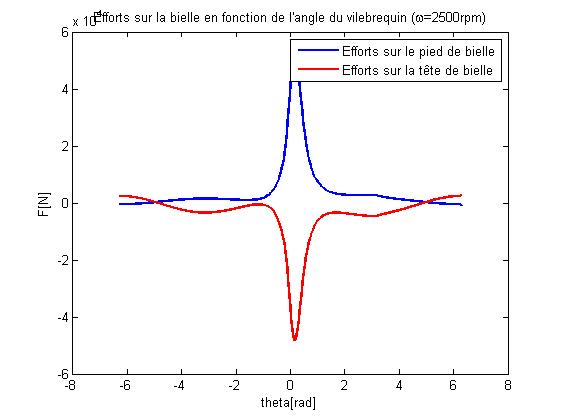
\includegraphics[scale=0.5]{effort_2500rpm.jpg}
\caption{Efforts lors d'un cycle, $\omega=2500rpm$}
   \end{minipage}\hfill
   \begin{minipage}[b]{0.48\linewidth}   
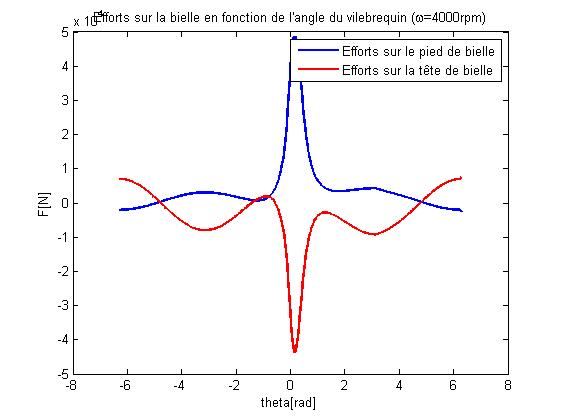
\includegraphics[scale=0.5]{effort_4000rpm.jpg}
\caption{Efforts lors d'un cycle, $\omega=4000rpm$}
   \end{minipage}
\end{figure}

Les efforts maximaux et minimaux à ces deux vitesses sont repris dans les tableaux ci-dessous: \\

\begin{figure}[h!]
\begin{center}
\begin{tabular}{|c||c|c|}
\hline 
\ & Forces maximales [kN] & Forces minimales [kN] \\ 
\hline 
Pied de la bielle & 50.225 & -0.995 \\ 
\hline 
Tête de la bielle & 2.931 & -48.313 \\ 
\hline 
\end{tabular} \\
\end{center}
\caption{Efforts maximaux et minimaux, $\omega=2500rpm$}
\end{figure}

\begin{figure}[h!]
\begin{center}
\begin{tabular}{|c||c|c|}
\hline 
\ & Forces maximales [kN] & Forces minimales [kN] \\ 
\hline 
Pied de la bielle & 48.692 & -2.547 \\ 
\hline 
Tête de la bielle &  7.503 & -43.798 \\ 
\hline 
\end{tabular} \\
\caption{Efforts maximaux et minimaux, $\omega=4000rpm$}
\end{center}
\end{figure}

\section{Justification de la forme de la bielle}

 Pour le corps de la bielle, il faut trouver le juste compromis entre masse et résistance. Pour une même forme de section, une augmentation de sa taille va de pair avec une hausse de la résistance et du poids de la bielle. La section profilée en I permet une résistance élevée au flambage tout en conservant une masse moins importante. Nous pouvons déterminer la force critique d'une poutre profilée en I grâce à la formule d'Euler : $F_{crit}$ = $\frac{\pi^2 *E*I}{(l_k)^2}$ où E est le module de Young, I le moment quadratique de la bielle et $l_k$ est la longueur de flambage de la poutre. Le module de Young étant propre au matériau et $l_k$ l'entraxe de la bielle, le seul moyen de maximiser la force à partir de laquelle apparaitra le flambage est de trouver la forme pour laquelle le moment quadratique [unité: $m^4$] est maximal. Voici la formule du moment quadratique d'une poutre profilée en I : $\frac{t}{6}*h^3*(1+\frac{3s}{h})$ où t est la demi-largeur de l'âme, s la largeur de la semelle et h la hauteur de l'âme. Ces distances sont annotées dans le dessin suivant\footnote{\url{http://fr.wikipedia.org/wiki/\%C3\%82me_\%28poutre\%29}}:
 \begin{figure}[H]
\center
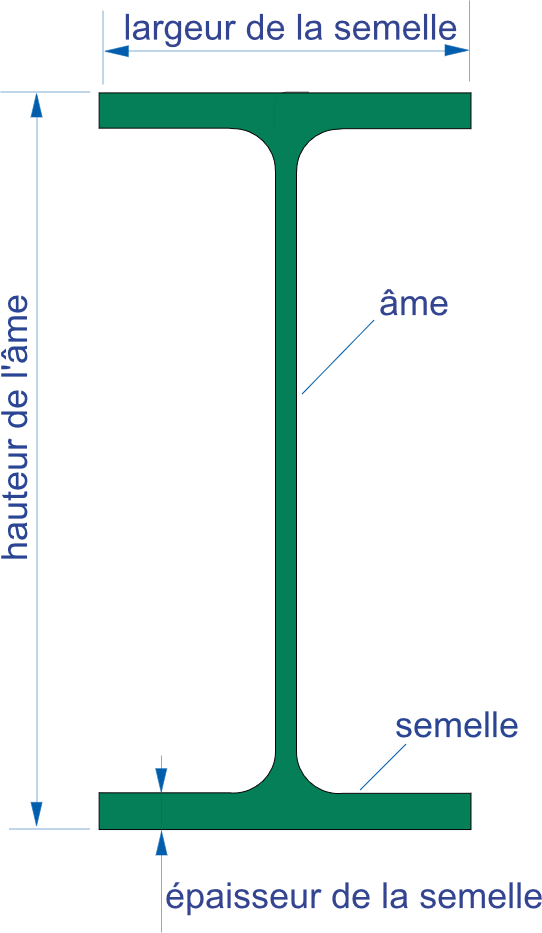
\includegraphics[scale=0.15]{Poutrelle.png}
\caption{Poutre profilée en I}
\end{figure}

\section{Dimensionnement de la bielle}

Il s'agit maintenant de déterminer les dimensions de la section profilée I du corps de la bielle. On sait grâce à la question 3, que la force maximale subie par la bielle au cours d'un cycle vaut 56,195 kN. Cette force étant celle à partir de laquelle la bielle est sujette au flambage, il faut prévoir une marge de sécurité. Nous décidons arbitrairement de la fixer à 25\%. Grâce à cela, en utilisant la formule d'Euler nous pouvons isoler le moment quadratique. Puisque nous supposons que la bielle a été obtenue par moulage, nous connaissons E (=170 000 MPa) et $l_k$ (=140,81 mm). Nous trouvons que $I = 8,301*10^{-10} [m^4]$. Enfin, en partant de la formule du moment quadratique d'une poutre profilée I, nous obtenons une équation liant hauteur d'âme, largeur de semelle et demi-largeur d'âme. On peut donc avec une assez grande liberté du choix des dimensions, déterminer ces 3 inconnues pour autant qu'elles soient réalistes ! (Par exemple, la hauteur d'âme ne peut pas être plus grande que le grand axe de l'ellipse du piston, sinon la bielle ne rentre plus dans le cylindre !)
Afin de déterminer ces trois inconnues, nous avons ajouté deux équations : $\frac{2*h}{3} = s$ et $2t=\frac{s}{4}$.

A titre de comparaison, voici les résultats mesurés et ceux dimensionnés :
(A noter que pour le calcul de l'aire de la section de la bielle dimensionnée, nous avons arbitrairement fixé l'épaisseur de la semelle comme égale à celle de l'âme.)
\begin{center}
\begin{tabular}{|c||c|c|}
\hline 
\ & Dimensions mesurées [mm]  & Dimensions calculées [mm] \\ 
\hline 
Hauteur d'âme & 23 & 11.88 \\ 
\hline 
Largeur de la semelle & 16.33 & 7.92 \\ 
\hline 
Epaisseur de l'âme & 3.8 & 1.98 \\
\hline
\end{tabular} \\
\end{center}
\begin{center}
\begin{tabular}{|c||c|c|}
\hline 
\ & Déterminée grâce aux mesures de séance $[mm^2]$ & Dimensionnée $[mm^2]$ \\
\hline
Aire de la section & 200,17  &  47,05 \\
\end{tabular}
\end{center}

On observe que les dimensions réelles sont très proches du double de nos prévisions. Cela peut s'expliquer de plusieurs manières: il est fort probable que le constructeur a choisi de prendre une grande marge de sécurité pour assurer un bon fonctionnement dans des conditions réelles, plus difficiles. De plus, la sécurité à une grande importance dans le secteur de l'automobile. On peut aussi estimer que le raisonnement suivi pour aboutir à nos résultats était simplifié et ne prenait pas compte de tous les paramètres, ce qui peut fausser les résultats.

\chapter{Annexe}

\section{Code Matlab}

\end{document}